\chapter{Introduction} % Main chapter title

\label{Chapter1} % Change X to a consecutive number; for referencing this chapter elsewhere, use \ref{ChapterX}

In this chapter a first introduction \ldots

\section{Context}

%Explicar que es SAT, la logica, boolean formula, pseudo boolean, cnf , satsolvers, minimization\\
%Target audience: logic researchers, planners etc...\\
%Users: C++ programmers which works with logic and want to represent their formulas and improve their time\\
%Beneficiaries:\\
\textbf{Boolean satisfiability problems} \textit{(SAT from now on)} is the problem of finding a model\footnote{An interpretation which satisfies the formula.} for a \emph{Boolean Formula}. In other words, it is the result of evaluating the \emph{Boolean Formula} after replacing its variables for \emph{true} or \emph{false}. 
\\
\emph{SAT} is widely used in Computer Science because it was the first problem proved to be NP-Complete\cite{Cook1971}\footnote{NP and NP-hard.} which allowed a lot of NP\footnote{Nondeterministic polynomial time.} to be reduced to it.

\subsection{What is a Pseudo-Boolean Formula?}
In propositional logic, a boolean formula is defined as following\cite{Lpo}:\\
Let $P$ be a set of predicate symbols like $p,q,r,...$
\begin{itemize}
	\item All predicate symbol of $P$ is a formula.
	\item If $F$ and $G$ are formulae, then $(F \land G)$ and $(F \lor G)$ are formulae to.
	\item If $F$ is a formula, then $(\neg F)$ is a formula.
	\item Nothing else is a formula.
\end{itemize}
This representation has some limitations because it can only express properties which are \emph{true} or \emph{false}.\\


\section{Background}

During the past semester (Q1 2017/2018) I had been developing a C++ library called \_\_\_\_\_.\\
This tool allows the users to represent \emph{Boolean Formulas} in a C++ program in a intuitive way, do operations between them and convert them into \emph{BDDs}. However, the main functionality of this library is the conversion from a \emph{Boolean Formula} to a \emph{CNF}.  \\
As previously explained, \emph{CNF} is a particular type of a \emph{Boolean Formula}, a conjunction of disjunctions. \emph{CNF} is an important format because it is the standard input for \emph{SAT Solvers}\ref{A.1}.\\
As shown in this paper, \emph{Mitchell, Selman, and Levesque\cite{Mitchell}}, there is a correlation between the number of variables, the number of clauses and the hardness of solving the \emph{CNF}.
\begin{center}
	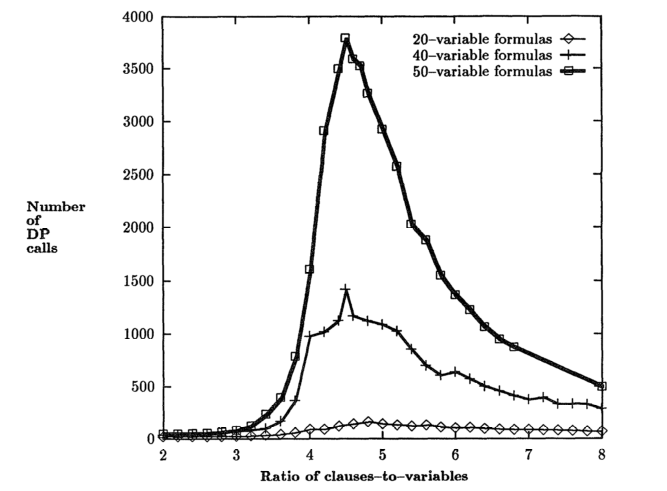
\includegraphics[width=1\textwidth]{Figures/GraphMitchellSelmanLevesque.png}
	\captionof{figure}{Median number of recursive DP calls for Random 3-SAT formulas, as a function of the ratio of clauses-to-variables. \\Extracted from Mitchell, Selman, and Levesque\cite{Mitchell}}
\end{center}
Therefore, an improvement of the input \emph{CNF} of the \emph{SAT Solver} can reduce a lot the hardness of the problem. \\
This is the main goal of the library, try to reduce the size of the final \emph{CNF} resulting from applying different converting methods on the original \emph{Boolean Formula}.

\section{Sate-of-art}

%Parlar d'alguns papers anteriors i discutirlos una mica per sobre

\section{Motivation}

\href{https://www.fib.upc.edu/en/studies/bachelors-degrees/bachelor-degree-informatics-engineering/curriculum/syllabus/LI}{Informatics Logic} is taught in this\footnote{\href{https://www.fib.upc.edu/en/}{Facultat Informàtica de Barcelona}} faculty. In that course I realized how important is \emph{logic} through its lecturer, \href{http://www.lsi.upc.es/~roberto/}{Dr.Robert Nieuwenhuis}, and its activities. \\

In the first coursework we had to code a \emph{SAT Solver} which used \emph{Unit Propagation}\ref{A.2}. With this activity I comprehended how hard and substantial is the study of \emph{logic} and all its context. For example, how \emph{logic} is used in Artificial Intelligence and Planners.\\

When the time of deciding the \emph{TFG} arrived, I contacted my actual supervisor, \href{https://www.cs.upc.edu/~jordicf/}{Dr. Jordi Cortadella}, and he proposed me some topics and ideas for projects. Finally, we agreed on doing this project. 
